\documentclass{article}
\usepackage{graphicx}
 \graphicspath{{./downloads/}}
 \usepackage{url}

\title{MM20B017 - DIVYA JYOTHI D}
\begin{document}
\date{}
\maketitle


\section{The Equation}

 {\huge $f(x)= \frac{1}{\sigma \sqrt{2\pi}} e^-\frac{1}{2}(\frac{x-\mu}{\sigma})^2$}
 \\
\\Variables:
\\$f(x) = probability \ density \ function$
 \\ $\sigma = standard \ deviation $
 \\$ \mu = mean$
 \\ $\pi \ \approx 3.14159... $
 \\ e $\approx$ 2.71828...
 \section{Description}
 The above is the equation for normal distribution or probability density function.It is also called as the equation of \textbf {Bell Curve} or the \textbf{Gaussian Equation} named after the scientist {\emph{Carl Friedrich Gauss}}. This equation can be used to express any bell curve as a function of x.This equation is used to represent the probability density distribution of a normally distributed random variable.
 \\Let us consider a case where tiny steel balls in a container are made to pass through a narrow neck separating the container into two halves.The situation is illustrated in fig.1 below. \\
 
 \begin{figure}[htbp]
    \centerline{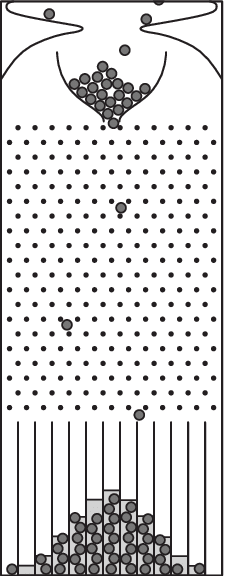
\includegraphics[width=6cm]{curve.png}}
    \caption{Illustration of the above case}
    \label{fig:mesh1}
\end{figure}

The tiny steel balls from the top half fall through the narrow neck into the bottom chamber. Observe that the number of balls collecting at the centre is maximum and it gradually diminishes towards the sides giving rise to a bell-shaped profile.
 \\ This shows that the probability of a random variable occurring at its mean value is maximum and diminishes for values away from the mean.
 \cite{enwiki:1026848272}
 \cite{article}
 \newpage
\bibliographystyle{plain}
\bibliography{mm20b017}
\end{document}
 
